\documentclass[tikz, border=10pt]{standalone}
\usepackage{tikz}
\usetikzlibrary{angles, quotes}

\begin{document}
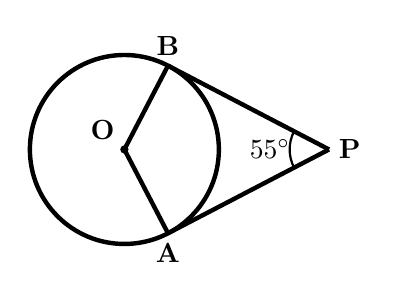
\begin{tikzpicture}

% Define radius
\def\r{1.2}

% For angle BPA = 55°, half angle = 27.5°
% Distance OP = r / sin(27.5°)
\pgfmathsetmacro{\d}{\r/sin(27.5)}

% Define center O
\coordinate (O) at (0,0);

% Define point P outside the circle (on the right)
\coordinate (P) at (\d, 0);

% Define tangent points on circle
% B at angle 62.5° (upper tangent point)
% A at angle -62.5° (lower tangent point)
\coordinate (B) at (62.5:\r);
\coordinate (A) at (-62.5:\r);

% Draw the circle
\draw[ultra thick] (O) circle (\r);

% Draw tangent line from P to B
\draw[ultra thick] (P) -- (B);

% Draw tangent line from P to A
\draw[ultra thick] (P) -- (A);
\draw[ultra thick] (B) -- (O);
\draw[ultra thick] (A) -- (O);

% Draw angle arc at P (55°)
\pic[draw, thick, angle radius=0.5cm, angle eccentricity=1.5, "$55^{\circ}$"] {angle=B--P--A};

% Label points
\node[above] at (B) {\textbf{B}};
\node[below] at (A) {\textbf{A}};
\node[right] at (P) {\textbf{P}};
\node[above left] at (O) {\textbf{O}};

% Draw filled dot at center O
\fill (O) circle (1.5pt);

\end{tikzpicture}
\end{document}